\documentclass[11pt]{article}

%----------Packages----------
%These are packages that give LaTeX more functionality
\usepackage{amsmath}
\usepackage{amsthm}
\usepackage{fullpage}  %%smaller margins
\usepackage{graphicx}
\usepackage{float}

%----------Theorems----------
%These are "theorem environments" which all look like a mathematical theorem (in terms of formatting).

%See what happens if you comment out this first line.
\theoremstyle{definition}
%The first {} is the name of the environment we use when creating one.
%The second {} is the name that appears when we use it.
%The [section] command tells LaTeX to number the theorems based on what section they are in.
\newtheorem{theorem}{Theorem}[section]

%the [theorem] option in the following lines tells LaTeX to use the same numbering system for theorems, propositions, definitions, and questions (but not remarks).
\newtheorem{proposition}[theorem]{Proposition}
\newtheorem{definition}[theorem]{Definition}
\newtheorem*{remark}{Remark}
\newtheorem{question}[theorem]{Question}

%I like to use this custom title header for classroom documents instead of the standard \title and \author. The \newcommand creates a new function which I have called \head. The [1] says that it takes one parameter. Everything between the outermost {...} is what the command actually does.
\newcommand{\head}[1]{
	\begin{center}         %Center the text
		{\large #1}        %The #1 refers to the first input parameter. It makes all that text large
	\end{center}
	\bigskip               %This adds some vertical space. Try removing it.
}


%Try changing this number and see if you can spot the effect.
%Try changing 'section' to 'subsection'.
%Try removing this line altogether.
\setcounter{section}{1}


\begin{document} 

%Here I use my custom \head command in place of \maketitle
\head{Let's Learn \LaTeX\\
Level 2\\
URSI 2025\\
Trevor Hyde
}

%Sometimes I don't want a big section header for my introduction, so I'll use \subsection instead. The \setcounter command in the preamble helps make the numbering work the way I want.
\subsection{Introduction}

%I like to put every sentence on its own line, but this is just a matter of personal style. The reason I do this is because in most LaTeX editors, you can double click on the .pdf at any point and then automatically jump to the corresponding line in the .tex file. If an entire paragraph is written on one line, then double clicking on a sentence in this paragraph will only take you to that paragraph instead of the line you want. Also, having each sentence on its own line makes it more convenient to comment out an entire sentence.
We can use \textit{environments} to create sections of our document with special, consistent formatting.
For example, in mathematics we have formal definitions, questions, remarks, propositions, lemmas, theorems, and proofs.
Here are some examples of what these look like in action.


\begin{question}
    How much wood would a woodchuck chuck if a woodchuck would chuck wood?
\end{question}

\begin{definition}
    For $t \geq 0$, let $W(t)$ denote the mass in kilograms of wood chucked by an average wood chuck who would chuck wood $t$ minutes after being provided with wood.
\end{definition}

\begin{proposition}
    Provided that the woodchuck would chuck wood, we have
    \[
        W(t) \geq 3t + 1
    \]
\end{proposition}

\begin{proof}
    It is well-known that every woodchucking woodchuck reflexively chucks a kilogram of wood immediately when provided with at least as much wood.
    \footnote{In fact, this reflexive chuck is documented to be so accurate and precise at measuring one kilogram that there has been some discussion at NIST of utilizing the woodchuck as an efficient means for distributing woodchucks as an efficient way to standardize the kilogram.
    The only challenge is to find enough woodchucks who \textit{would} chuck wood.}
    %Here we cite a source listed in our bibliography. There are several ways to include a bibliography in a LaTeX file, the simplest is to include it at the bottom of your file using the bibliography environment. More details on how this works may be found below.
    According to \cite{FP11}, the average instantaneous woodchucking rate $W'(t)$ is bounded below by $3$ kg/min.
    Hence
    %The proof environment ends with the traditional empty square symbol \qed. However, if we end our proof on a math display line, then the \qed symbol appears awkwardly below the end of our display line. To fix this we can use the \qedhere command, which puts the \qed symbol at the end of the math display line instead of where it would normally go.
    \[
        W(t) \geq 1 + \int_0^t 3\,dx = 1 + 3t.\qedhere
    \]
\end{proof}

We often want to include tables of data in our files.
This can be accomplished with the \texttt{tabular} environment.

%The [h] determines the placement of the table on the page. It tells LaTeX to put the table right here instead of choosing a placement that fits more efficiently.
\begin{table}[h]
    %%The centering command makes everything in this table environment centered on the page.
    \centering
    %The tabular environment creates the table. The {|c||l|c|r|} describes the columns, their alignment, and the vertical bars between them. Experiment with changing this to see what happens to the table. 
    \begin{tabular}{|c||l|c|||r|} 
        %To add horizontal lines to our table, we use the \hline command.
        \hline
        %Within a given row, we use the & symbol to separate the columns. We need to have as many columns as are there are letters listed in our description of the columns. So 4 columns means we need 3 & per row. The \\ symbol means "end of row"
        Index & Name & Widget Code & Viscosity \\
        \hline
        0 & Pickle & \texttt{3@6L} & 0.01\\
        1 & Digit & \texttt{W;B2} & 0.899\\
        2 & Tire & \texttt{Q2Q>} & 0.11\\
        3 & Candelabra & \texttt{DDD9} & 0.32\\
        %There are certain symbols that have special meaning in LaTeX. If you try to type them directly, LaTeX gets mad. If this happens, you can put a backslash \ in front of the symbol. This is called an "escape character", which tells LaTeX to interpret what it sees next literally instead of as having a special meaning.
        4 & Rent & \texttt{\_M3\&} & 0.2\\
        \hline
    \end{tabular}
    %Captions are optional, but this is how you make them.
    \caption{Important widget data}
    %Labels are also optional. They help you refer back to the table later.
    \label{table: my important widget data}
\end{table}

\begin{remark}
    %I like to indent text within an environment to help keep the LaTeX file legible, but this is not necessary.
    %Here we use the label on our table to refer to it. This is much better than typing the number of the table directly, since if you later add more tables above this, all the numberings will be automatically updated. It's a pain to update manually!
    Table \ref{table: my important widget data} contains important widget data. Everyone should commit it to memory.
    See \cite{JK25} for more info.
\end{remark}

Typing out a table by hand can be annoying, especially if it is large.
There are a few shortcuts we can take in our advanced modern age. 
In Overleaf, there is a toolbar at the top of the editing window which contains a table button that allows you to automatically generate a table of any prescribed size.
I never use this, but it's an available option.

Another option which I like more is to use generative AI to create the table I'm looking for.
If you know roughly what you want the table to look like, you can sketch out a mock up, take a picture, upload it to your favorite chatbot, and ask for the code in LaTeX.
This works best if you include a detailed description of how it should look.

For example, let's say I want to make a table which shows the first few square and triangular numbers.
Here is a sketch of the table I want.
\begin{center}
    %To include pictures into your files, you can use the \includegraphics command. I like to keep all my pictures in a folder to keep my projects organized. Here I have labelled this folder figs. In the square brackets we include optional parameters, like scale. Often images are way too big, so it is necessary to scale them down.
    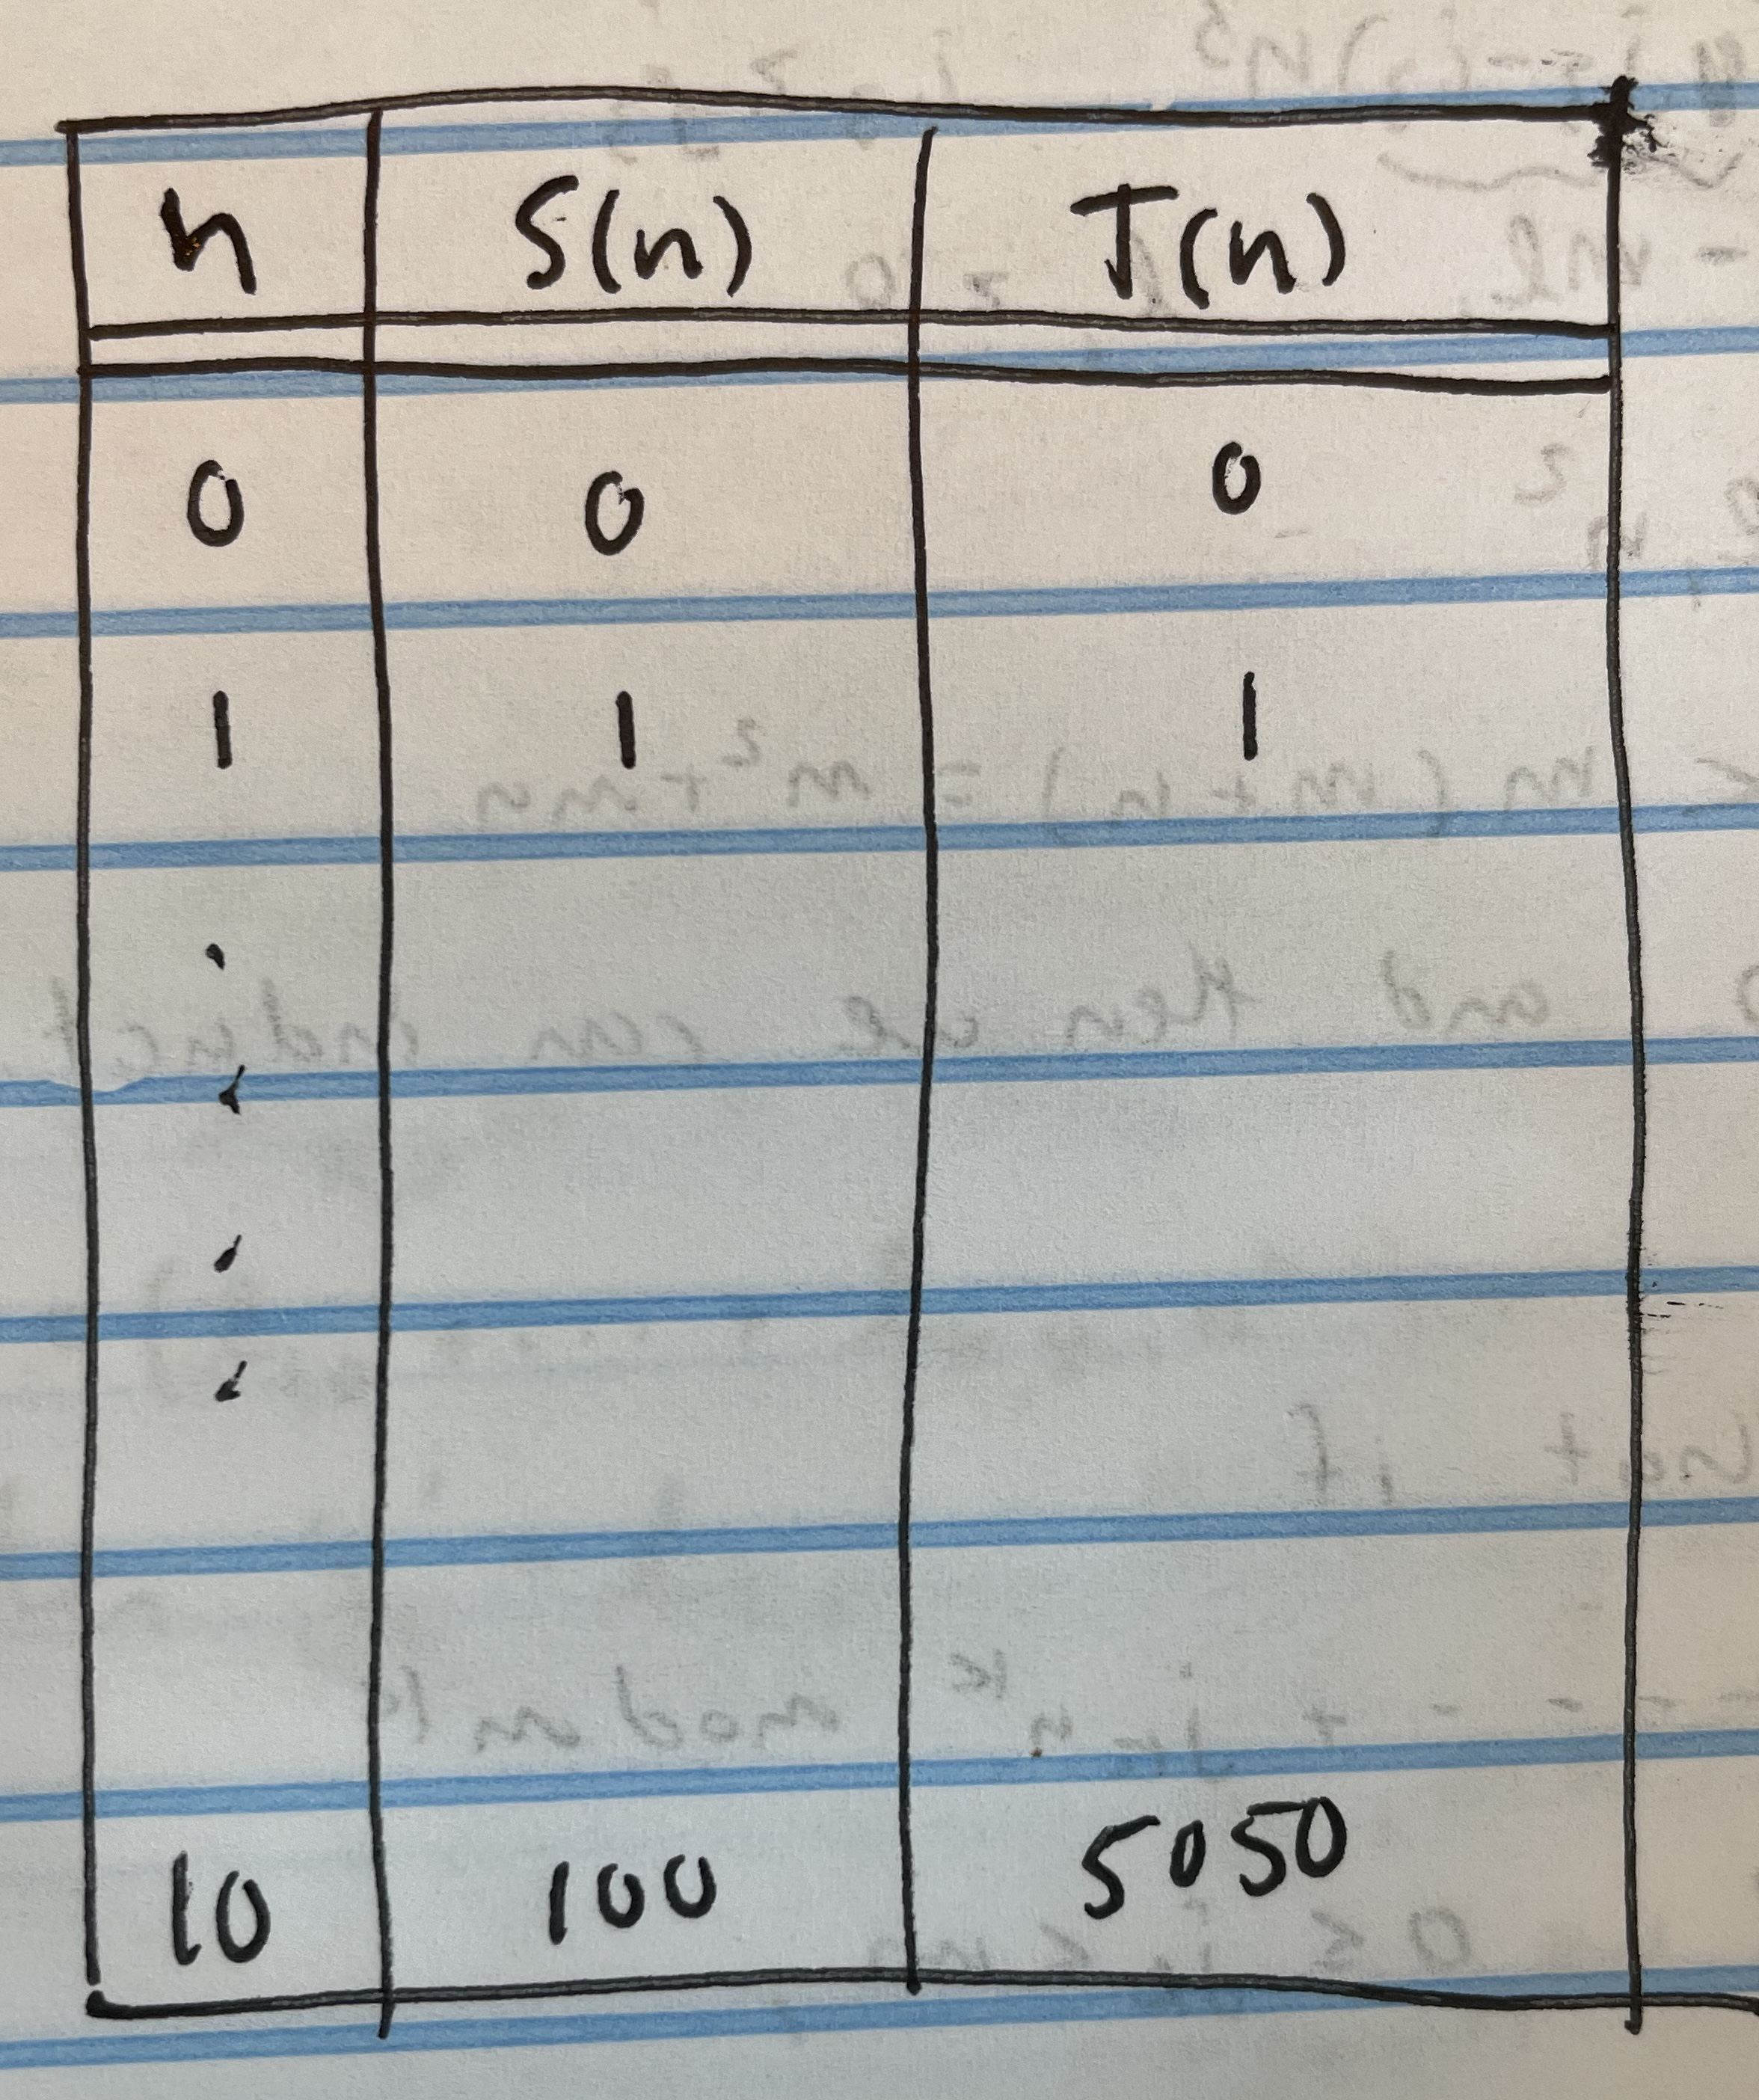
\includegraphics[scale=.06]{figs/table_sketch.jpeg}
\end{center}
I uploaded this to Gemini with the prompt:
%The quote environment indents text and seperates them from their surroundings with some space.
\begin{quote}
    Can you generate the code for a LaTeX table for me that looks like the one in this sketch? There should be 11 rows labeled 0 through 10. Let n denote the label on each row. In the second column list the value $n^2$. In the third column list the nth triangle number.
\end{quote}

After briefly inspecting the numbers to make sure they were correct, I pasted the code it gave me into this file and got this table.

\begin{center}
    \begin{tabular}{|c|c|c|}
        \hline
        $n$ & $S(n)$ & $T(n)$ \\
        \hline
        0 & 0 & 0 \\
        \hline
        1 & 1 & 1 \\
        \hline
        2 & 4 & 3 \\
        \hline
        3 & 9 & 6 \\
        \hline
        4 & 16 & 10 \\
        \hline
        5 & 25 & 15 \\
        \hline
        6 & 36 & 21 \\
        \hline
        7 & 49 & 28 \\
        \hline
        8 & 64 & 36 \\
        \hline
        9 & 81 & 45 \\
        \hline
        10 & 100 & 55 \\
        \hline
    \end{tabular}
\end{center}

%This command creates a bibliography. The first FP11 is the longest bibliography label. It tells the environment how much to indent everything by. You can try changing it to see the effect.
\begin{thebibliography}{FP11}
    %\bibitem creates an entry in our bibliography. The text in brackets [] will be the label we see at the start of each row. The text in {} is the label we can use to refer to this entry. Note that they don't have to be the same but often are.
    \bibitem[FP11]{FP11}
    J. Fennel, P. Pipstein, Chuck this out: liminal woodchucking rates, \emph{Chucking Quarterly}, \textbf{159}, no. 11 (2011)

    \bibitem[JK]{JK25}
    F. Jones, S. Kornwall, Essential widget viscosity, \emph{Journal of the American Widget Society}, \textbf{77}, no. 3 (2024) 
\end{thebibliography}

\end{document}

